\chapter{The ATLAS Detector}
\label{chap:detector}

\epigraph{Scientific apparatus offers a window to knowledge, but as
  they grow more elaborate, scientists spend ever more time washing
  the windows.}{Isaac Asimov}

The ATLAS experiment is one of the four large experiments at the Large
Hadron Collider (LHC) located at the European
Council for Nuclear Research (CERN) outside of Geneva,
Switzerland. Buried between 45 m and 170 m under the French-Swiss
border, the LHC accelerates two counter-rotating beams of protons to
$4 \tev$ each. The proton beams are steered with superconducting
magnets around an
evacuated ring that is 26.7 km in circumference~\cite{bib:Evans:2008zzb}. At several points along
the ring, the beams are steered and focused such that the constituent
protons collide with high probability at a center-of-mass energy of $8
\tev$. One such point is surrounded by the ATLAS detector, a
general-purpose detector designed to take a snapshot of the collision
remnants~\cite{bib:Aad:2008zzm}. In this chapter, the various subsystems of the ATLAS
detector are discussed, and in the following chapter, the
reconstruction of a $pp$ collision from the ATLAS readout channels is
considered. 

\section{Overview}
\label{chapter:detector:section:overview}

The ATLAS detector is situated along the LHC beam pipe. Its global
coordinate
system is defined with the $z$ coordinate coinciding with the
direction of
the proton beam, $x$ pointing towards the center of the
LHC ring, and $y$ pointing upwards. The azimuthal angle $\phi$ is the
angle in the $x-y$ plane as measured from the $x$ axis, and the polar
angle $\theta$ is the angle from the $z$ axis. The origin of this
coordinate system lies nominally at the center-of-mass of the
detector, though in particle reconstruction, it is shifted to be the
$pp$ collision point. In most cases, the $\theta$ coordinated is
replaced by the pseudo-rapidity, defined as $\eta = -\log (\tan
(\theta/2))$, because for massless particles this quantity is Lorentz
invariant with respect to boosts in the $z$ direction. Detector
components or particles near the beam axis, considered to be
``forward'', lie at large values of $|\eta|$.

ATLAS is designed to be sensitive to the broad range of scattering
events expected at the $\tev$ scale. One of the primary design
considerations was the search for the Higgs boson. Since many Higgs
final states include charged leptons, a high precision tracking system
was required. Moreover, the $H\rightarrow{\gamma\gamma}$ channel calls
for robust EM calorimetry to identify and measure electrons and
photons. Another equally important consideration in the design was the
high expected LHC collision rate and the large QCD backgrounds
expected at a $pp$ collider. At its design luminosity, the collision
rate of the LHC is 1 GHz. The proton beam is partitioned into
\textapprox{3000} bunches with up to $10^{11}$ protons per
bunch, making it likely that more than one proton collision occurs
every time two bunches cross paths. Also, because the bunches are
separated by 25 ns, particles from adjacent bunches may appear to be
from the colliding bunch. These two phenomena, referred to as pile-up,
also shaped the design of ATLAS. To deal with these overlapping
events, the ATLAS components have fast recovery times and fine
granularity. Also, the
tracking system close to the collision region has high resolution,
allowing overlapping collisions to be distinguished in
reconstruction.

\begin{figure}[ht]
    \centering
    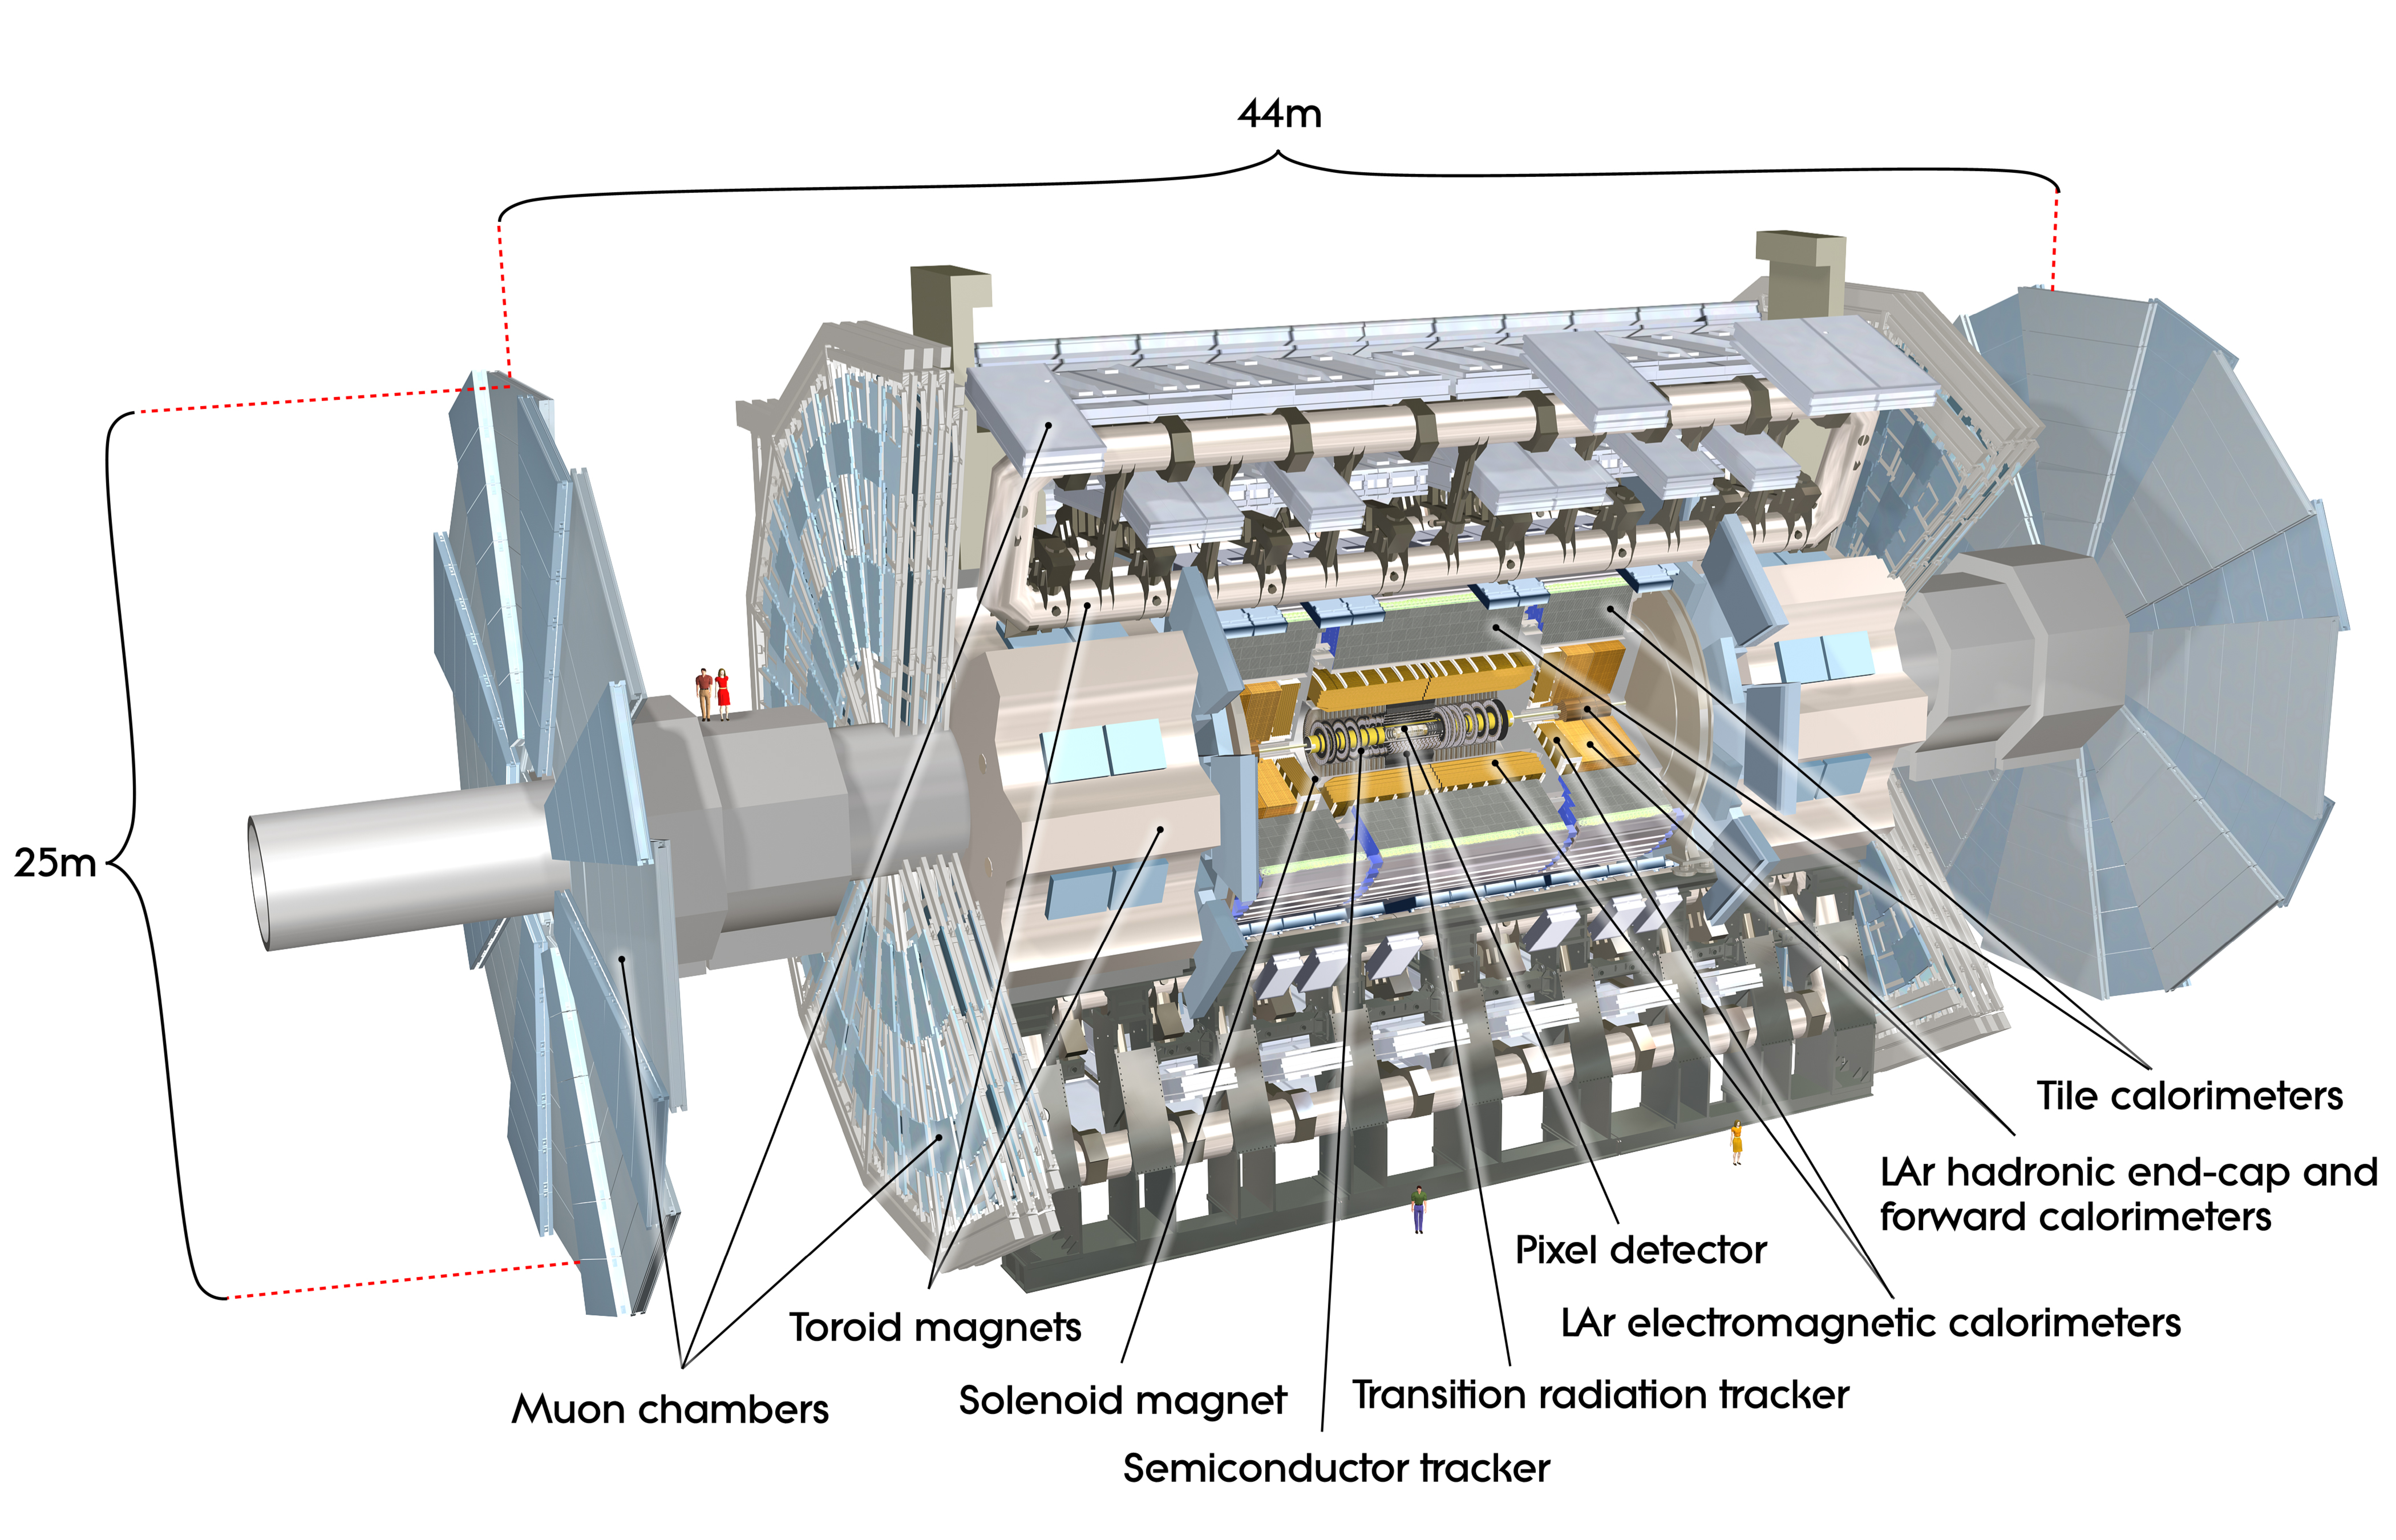
\includegraphics[width=1.0\textwidth]{fig/detector/full_atlas.pdf}
    \caption[]{}
\label{chap:detector:fig:full_atlas}
\end{figure}

The resulting design of the ATLAS detector is displayed in
figure~\ref{chap:detector:fig:full_atlas}. Lying closest to the
collision point, the inner detector (ID) is the primary tracking
system. To resolve the momentum of charged particles, it is immersed
in a uniform 2 T magnetic field. Beyond the ID are the EM and hadronic
calorimeters which measure the energy photons, electrons, and hadrons
produced in the collision. The outermost detectors comprise the muon
spectrometer (MS) system. These detectors are embedded in a high-bend
toroidal magnetic field, resulting in precision tracking across a
large momentum range. The detector is nominally $\pm z$-symmetric and
has eight-fold azimuthal symmetry due to the toroid magnet system. The
various subsystems are segmented in the $z$ direction into a barrel
region with a concentric cylinder geometry, and two end-cap regions
with components that are ``wheels'' or ``disks'' which fit against the
barrel ends, thereby increasing acceptance. 


\section{Inner Detector}
\label{chapter:detector:section:inner_detector}

Charged particles produced in collisions traverse the ID,
depositing on sensors signals that are recorded as spatial coordinates. These
coordinates are then processed through a pattern recognition and
reconstruction algorithm to extract the particle tracks from which the
momentum four vectors are derived (see
section~\ref{chap:reco:sec:tracks}). The ID is designed to measure
tracks across a large momentum range, from $O(100 \mev)$ to $O(1
\tev)$, falling in the pseudorapidity range $|\eta| < 2.5$. It is composed of three
sub-detectors: the pixel tracker, the silicon microstrip tracker
(SCT), and the transition radiation tracker (TRT). A cross-sectional
diagram of the ID in the barrel region is shown in
figure~\ref{chap:detector:fig:inner_detector}.

\begin{figure}[ht]
    \centering
    \includegraphics[width=0.8\textwidth]{fig/detector/inner_detector.pdf}
    \caption[]{}
\label{chap:detector:fig:inner_detector}
\end{figure}

\subsection{Silicon Detectors}

With nearly 50 $pp$ collisions per beam crossing producing $O(1000)$
particles per second, the detectors near the collision point are
required to have high resolution, fine granularity, fast response, and
radiation hardness. These requirements are satisfied by the silicon
pixel detectors. The 1744 identical pixel sensors of the pixel tracker
are arranged in three concentric layers in the barrel region
(figure~\ref{chap:detector:fig:inner_detector}) and in three disks in
each end-cap. Each sensor is composed of \textapprox{47k} pixels of
size $50~\mu\textrm{m} \times 400~\mu\textrm{m}$, corresponding to 80M readout
channels. The intrinsic spatial resolution of each pixel is
$10~\mu\textrm{m} \times 115~\mu\textrm{m}$, and the sensor is placed
such
that the precision pixel direction is the global azimuthal direction
in which charged particles bend. Due to the high efficiency of the
pixel sensors, the average charged particle
track in the ID volume will result in three precision spatial
measurements from the pixel tracker. 

Beyond the pixel detector lies the second silicon sub-detector in the
ID, the SCT. Due to budgetary constraints, the SCT relies on more
traditional technologies at the cost of degraded detector precision. In the
barrel region, the SCT modules are tiled to form four concentric
layers (figure~\ref{chap:detector:fig:inner_detector}), while in each
end-cap, the modules form nine disks, amounting to a total of 4088
modules. Each barrel module is composed of four nearly square
(64.0~mm~$\times$~63.6~mm) silicon
sensors, each with 768 readout strips that are $22~\mu\textrm{m}$ in
width~\cite{bib:Abdesselam:2006wt}. Two sensors are placed
side-to-side--- with a 2 mm gap for readout electronics--- on top of a
thermal pyrolitic graphite substrate, which provides mechanical
support and the thermal conductivity necessary for cooling the
sensors. Another two sensors are placed on the other side of the
substrate, and displaced by an angle of 40 mrad. This stereo angle
configuration allows another spatial degree of freedom to be
measured ($z$ in barrel, $R$ in endcap). The end-cap sensors and
modules are similar except for adjustments to the dimensions. The
intrinsic resolution of the SCT is $17~\mu\textrm{m}$ in
the azimuthal direction, and the effective resolution in the $z$ ($R$)
direction in the barrel (endcap) is $580~\mu\textrm{m}$. An average
track in the ID volume will result in four precision spatial
measurements in the SCT. 

\subsection{Transition Radiation Tracker}

The TRT is the outermost sub-detector in the ID, spanning the region
$56~\textrm{cm} < R < 108~\textrm{cm}$ in the
barrel~\cite{bib:Abat:2008zzb}. It is a collection of polyimide-based
drift chamber tubes (straws) that are 4~mm in diameter. The tube wall is the high
voltage cathode composed of layers of polyimide, graphite-polyimide,
polyurethane, and a 0.2 \micron layer of aluminium to achieve the
requisite electrical and mechanical properties~\cite{bib:Aad:2008zzm}. The anode is a
31 \micron gold-plated tungsten wire running directly through the
center of the straw with a radial offset of less than
300 \micron. Each straw is filled with a gas mixture of 70\% Xe, 27\%
CO$_2$, and 3\% O$_2$. 

In the TRT barrel region, spanning $|\eta| < 1.0$, the TRT straws run
parallel to the beam axis. They are placed in carbon-fiber-shelled modules
in which the straws form uniform arrays with an average spacing of
6.6~mm. The straws in the module are 144~cm long. To accomodate high
particle multiplicity, the wires within each straw are electrically
disconnected at the straw center, allowing two independent measurements
from a single straw. At either end of the module, there is a high
voltage plate that couples to the straw walls and a front-end
electronics board. A gas inlet circulates CO$_2$ outside of the
straws, thereby preventing electrical discharges and the accumulation
of any leaked Xe. This gas bath also cools the straws by conducting
heat to the highly thermally-conductive shell of the module. With a
quadralateral prism geometry, the modules are
arranged into three concentric rings, each comprised of 32 modules. 

The TRT end-caps provide tracking in the region $1.0 < |\eta| <
2.0$. Each end-cap consists of two sets of wheels. The set closer to
the collision point is composed of 12 wheels, each with eight straw
layers spaced at a wire-to-wire distance of
8~mm~\cite{bib:Abat:2008zz}. The other wheel set
has only eight wheels and a layer spacing of 15~mm. In each wheel,
there are 768 straws of length 37~cm oriented radially outwards with
uniform azimuthal spacing. To achieve better uniformity in the number
of straws that are traversed, each successive wheel is rotated by
$3/8$ of the azimuthal spacing. Similar to the barrel modules, each
wheel is a self-contained unit in which CO$_2$ circulates around the
straws. 

In total, there are 52544 straws in the barrel and 122880 straws in each
end-cap. On average, a charged particle with a momentum greater than
$500 \mev$ and $|\eta| < 2.0$ will traverse 36 straws, except in the
transition region between the barrel and end-cap, $0.8 < |\eta| <
1.0$. Each straw is capable of providing a measurement of the distance
of closest approach in the plane perpindicular to the straw direction
at an intrinsic resolution of 130 \micron. Therefore, in the barrel
(end-cap), the TRT measures an $R-\phi$ ($z-\phi$) coordinate but no $z$
($R$) information. 

\note{I should probably include a paragraph on electron ID capability}


\section{Calorimetry}
\label{chapter:detector:section:calorimeter}

The ATLAS calorimeters are designed to efficiently capture, and
precisely measure, the energy of photons, electrons, and hadrons. They
are symmetric about the beam axis and extend beyond the ID to $|\eta|
= 4.9$~\cite{bib:Aad:2008zzm}. The electromagnetic calorimeter, optimized for electrons and
photons, is segmented into a barrel and two end-caps. Its barrel is
housed in a liquid argon cryostat. The two end-caps have separate
cryostats that also contain the hadronic end-cap calorimeter (HEC) and
the forward calorimeter (FCal). Beyond the barrel EM calorimeter is
the hadronic tile calorimeter. A drawing of entire calorimeter system is
displayed in figure~\ref{chap:detector:fig:calorimeter}.

\begin{figure}[ht]
    \centering
    \includegraphics[width=0.8\textwidth]{fig/detector/full_calorimeter.pdf}
    \caption[]{}
\label{chap:detector:fig:calorimeter}
\end{figure}

\subsection{Liquid argon electromagnetic calorimeter}

The barrel of the EM calorimeter spans the region $|\eta|<1.48$, and
is split into two halves at $\eta = 0$. Lead plates with an accordion
geometry provide the needed absorbing material. This geometry, shown
in figure~\ref{chap:detector:fig:accordion}, yields uniform azimuthal coverage and fast detector
response~\cite{bib:Aad:2008zzm}. The readout electrodes are positioned parallel to
the lead plates in the center of the gap between adjacent plates. Each electrode
consists of three layers of copper separated by a thin insulating layer of
polyimide. The outer layers are set to the high voltage potential, and the
inner layer carries the signal to the electronics by
capacitive coupling. These electrodes are etched in order to define
the granularity in the $R$ and $\eta$ directions. The $\phi$
granularity is set by the spacing of the electrodes and how they are
integrated into the front-end electronics~\cite{bib:Aubert:2005dh}. The calorimeter is
subdivided in $R$ into three regions of varying granularity, with the
finest granularity closest to the collision point. In both the $\phi$
and $\eta$ directions, the granularity in the middle layer is 0.025. On either side of
the electrode, the distance is 2.1~mm, corresponding to a drift
time of 250~ns at a nominal voltage of 2.0~kV. The total thickness of
the barrel calorimeter is at least 22 radiation lengths, increasing to 33 as $|\eta|$
increases. 

\begin{figure}[ht]
    \centering
    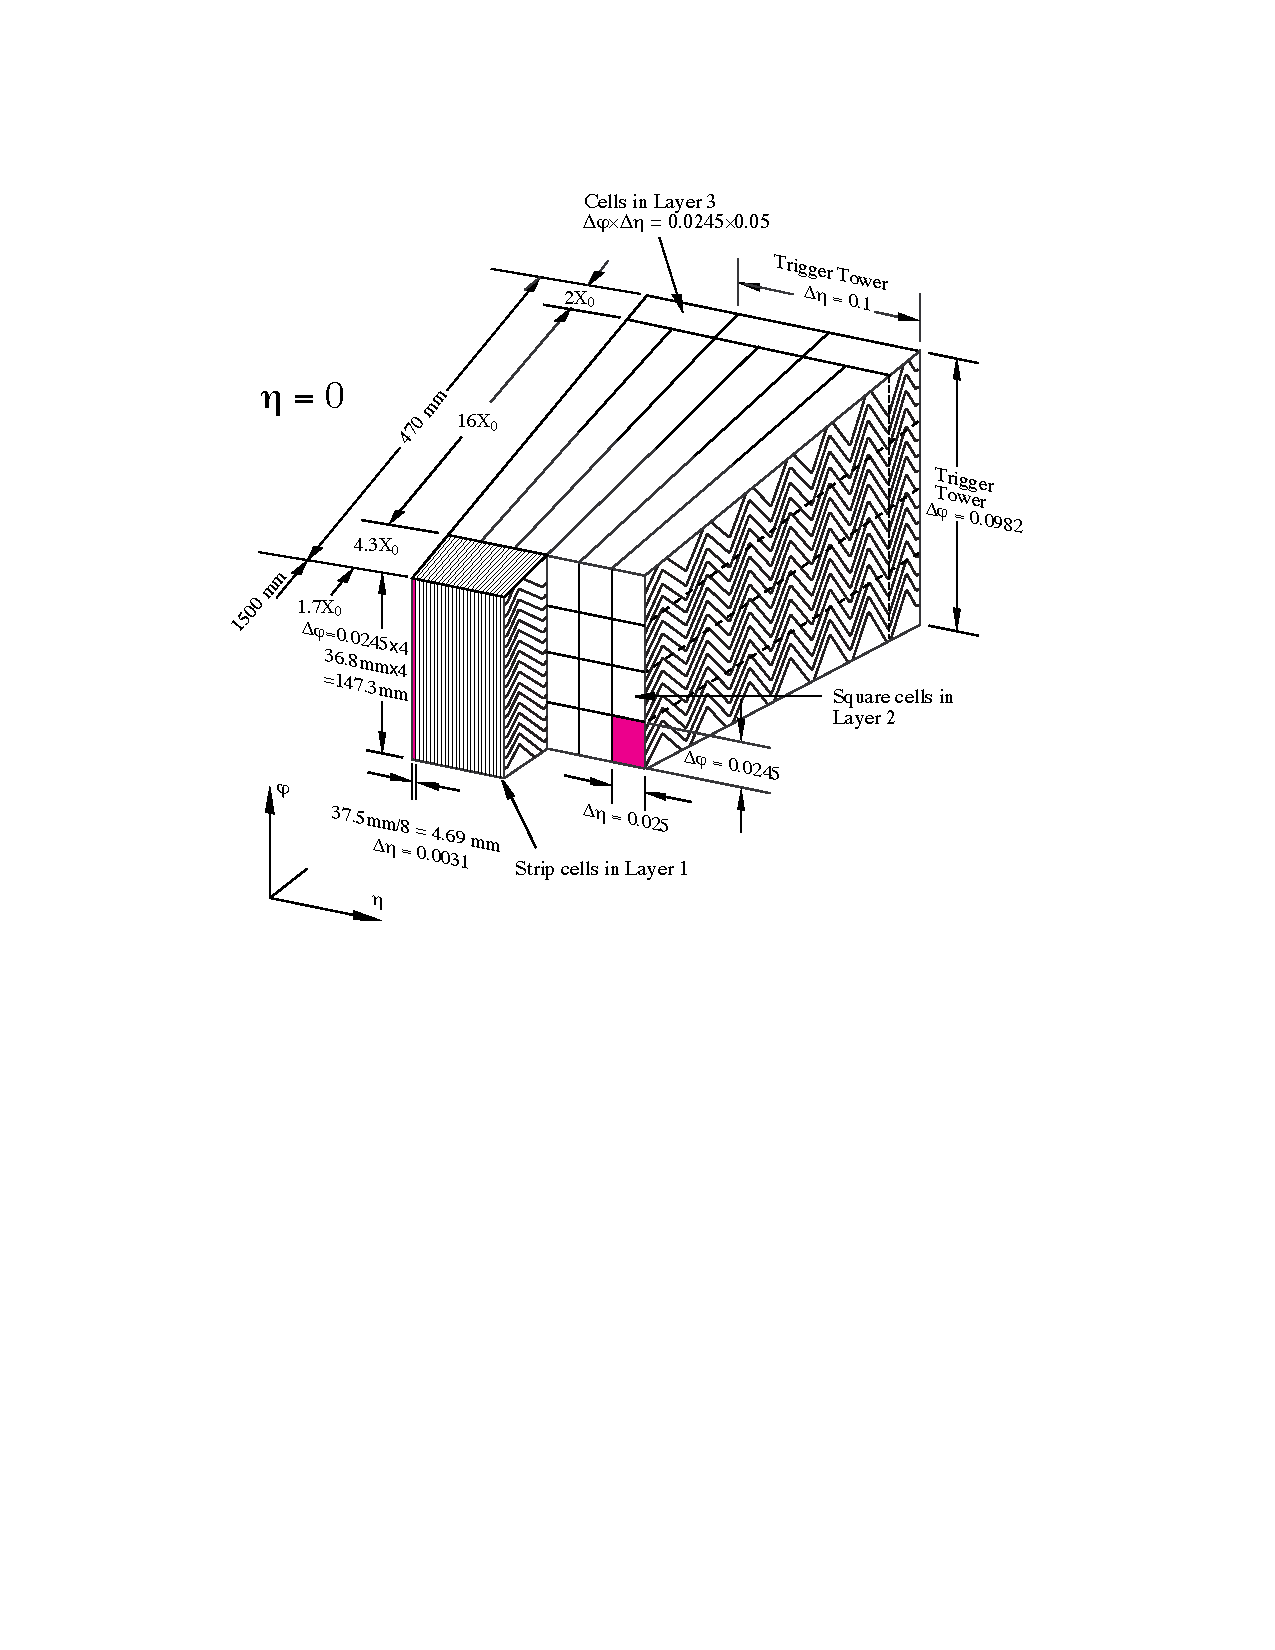
\includegraphics[width=0.7\textwidth]{fig/detector/em_calo_accordion.pdf}
    \caption[]{\cite{bib:Aad:2008zzm}}
\label{chap:detector:fig:accordion}
\end{figure}

The end-cap segments of the EM calorimeter cover the region
$1.38|\eta|<3.2$, with the overlap ensuring that there is no loss of
resolution in the barrel-end-cap transition region. Each end-cap is
segmented into two concentric wheels, with the inner (outer) wheel composed of
768 (256) lead plates. As for the barrel calorimeter, the plates are
accordion-shaped; however, in the end-cap, the perforations are in the
$R$ direction instead of the $z$ direction. The $R$-$\eta$
segmentation is set by etches in the inter-plate electrodes, forming
three layers of varying granularity, with a granularity of $\Delta\phi
\times \Delta\eta = 0.025 \times 0.025$ in the middle layer. The
thickness of the
end-cap calorimeter varies from 24 to 38 radiation lengths, depending on
$|\eta|$. 

Another important component of the EM calorimeter is the presampler,
located in front of the barrel calorimeter and just outside of the
solenoid coils~\cite{bib:Aad:2008zzm}. Spanning the region $|\eta| < 1.52$, the function of
the presampler is to collect the energy lost by incident particles
before reaching the calorimeter. This correction to the calorimeter
measurement improves the energy resolution by as much as
40\%~\cite{bib:Andrieux:2002xy}. The presampler provides full
azimuthal coverage with 32 modules of width $\Delta\phi = 0.2$ for
each half barrel of the calorimeter. It has a single active liquid
argon layer without any additional absorbing material. To collect
signal, sheets of electrodes are positioned parallel to the
$x$-$y$ plane. Two electrode types--- the anode and cathode--- are
interweaved to achieve a potential difference of 2.0 kV across the
active medium gap of 2~mm. The anode has the same three layer configuration as the
barrel and end-cap calorimeters, allowing the signal to be read out
by the central conductor. Each electrode is etched in the center to
give a $\phi$ granularity of 0.1. The desired $\eta$ granularity is
achieved by electrically connecting adjacent electrodes in the
longitudinal direction, resulting in a constant granularity of 0.025. 

\subsection{Hadronic calorimeters}

Hadrons from the $pp$ collision undergo nuclear interactions in the
detector material. Because these interactions occur at a low rate with
respect to the EM processes that produce energy in the EM calorimeter,
additional calorimeters with greater thickness are positioned beyond
the EM calorimeters. There are three types of hadronic calorimeters:
the barrel tile, the end-cap liquid argon, and the
forward liquid argon. 

The tile calorimeter is segmented into a barrel that covers the region
$|\eta| < 1.0$ and two extended barrels on either side, increasing the
coverage up to $|\eta| = 1.7$~\cite{bib:Abdallah:2008zz}. Each segment
is divided azimuthally into 64 modules. These modules house 4~mm and 5~mm
steel plates, oriented parallel to the $x$-$x$ plane, that act as the
absorbing material (figure~\ref{chap:detector:fig:tile_module}). In the gaps between plates, there are
polystyrene-based scintillating tiles of thickness
3~mm~\cite{bib:Aad:2008zzm}. Ionizing particles
crossing the tiles
produce high frequency visible light that is collected by optical fibers on
either side of the tile. The wavelength of the scintillation light is
shifted by the fibers that also carry the light to
photo-multiplier
tubes (PMTs) on the outer edge of the module, where it is converted to
an electrical signal. By grouping fibers together for
collection into the same PMT, the desired granularity is
obtained. These fiber groups form three layers in the $R$ direction,
with the first two having a granularity of $\Delta\phi
\times \Delta\eta = 0.1 \times 0.1$ and the third with $\Delta\phi
\times \Delta\eta = 0.1 \times 0.2$. The radial depth of the tile
calorimeter is approximately 7.4 nuclear interaction lengths. 

\begin{figure}[ht]
    \centering
    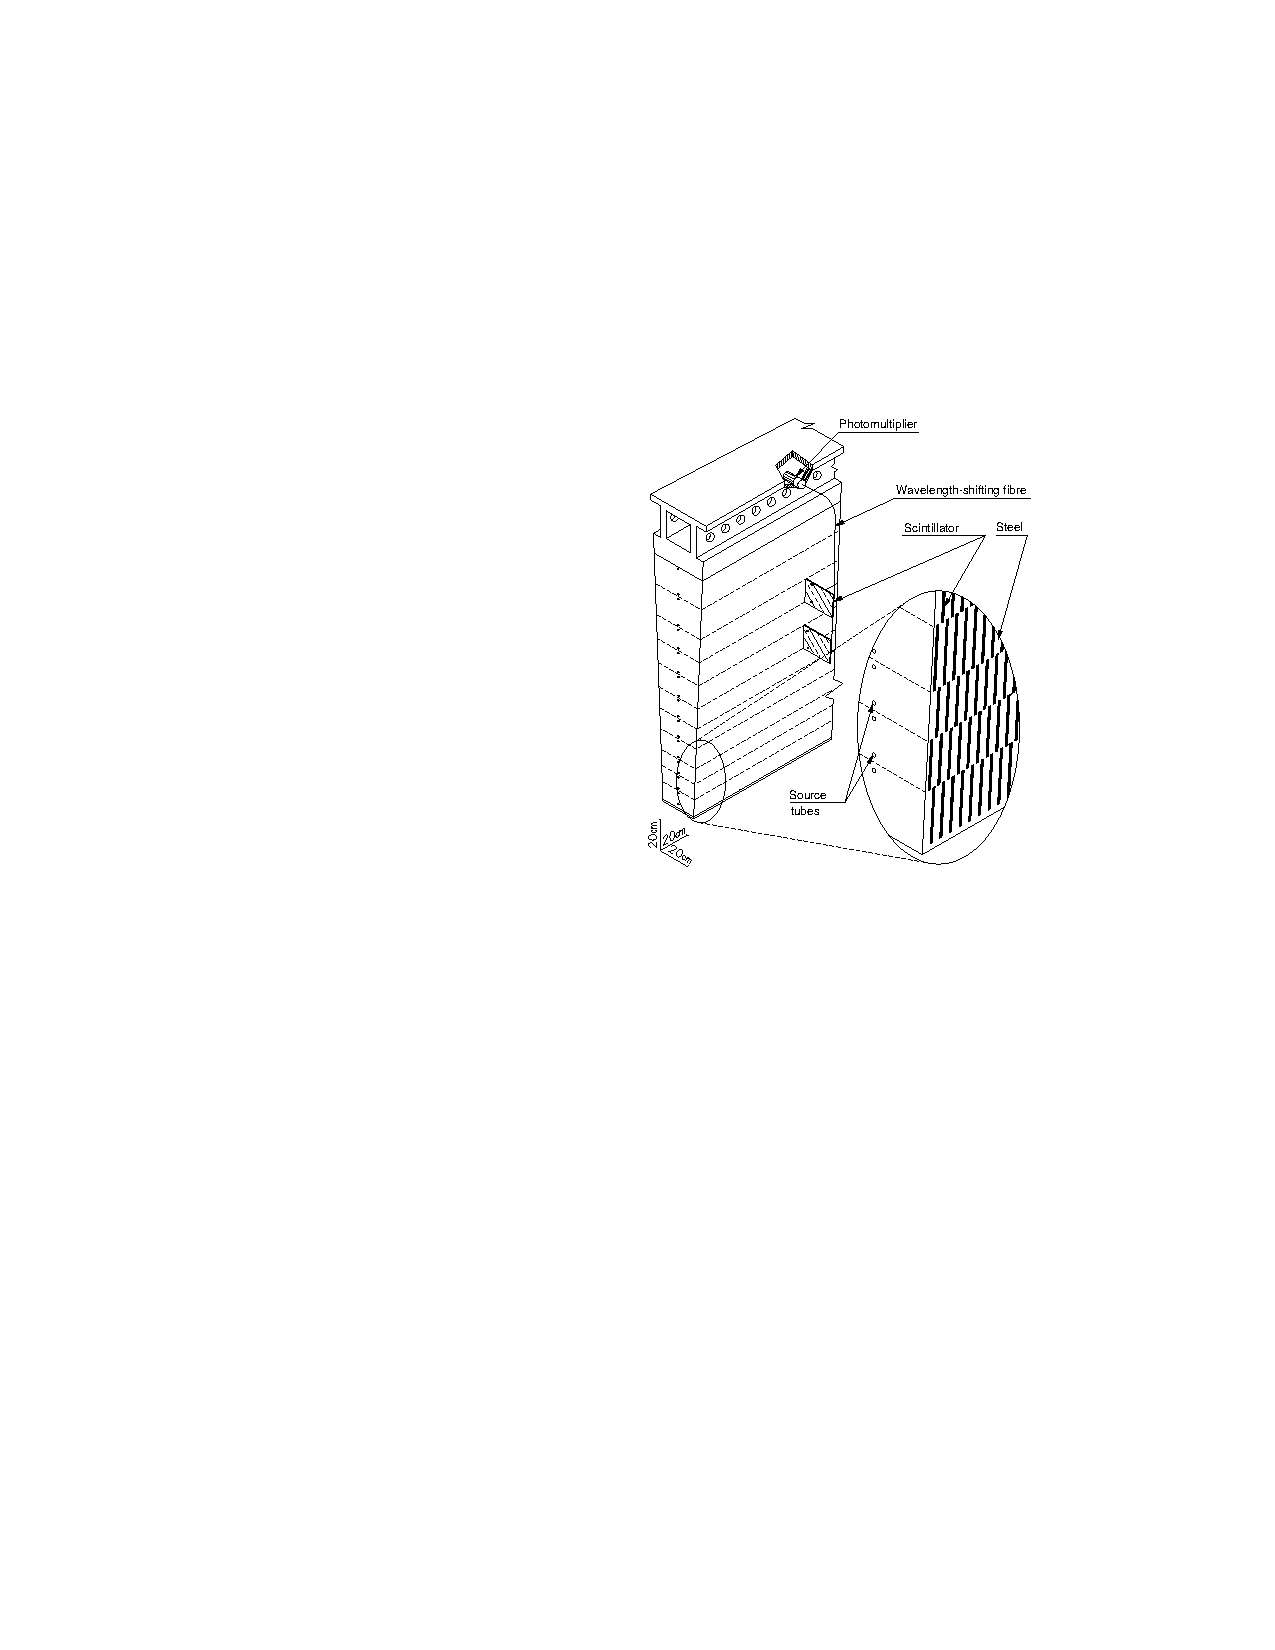
\includegraphics[width=0.5\textwidth]{fig/detector/tile_module.pdf}
    \caption[]{}
\label{chap:detector:fig:tile_module}
\end{figure}

The acceptance of the tile calorimeter is extended by the hadronic
end-cap calorimeter which spans the range $1.5 < |\eta| < 3.2$. Each
end-cap consists of two wheels with the same radius but positioned at
different $z$ values. Both wheels are partitioned in $\phi$ into 32
modules. In the inner (outer) wheel, each module contains 24 (16)
25~mm (50~mm) thick copper plates running parallel to eachother and to the
$x$-$y$ plane. The plates are separated by an 8.5~mm gap that is
further separated into four 1.8~mm liquid-argon-filled drift zones by
three electrodes. The central electrode is a 35 \micron sheet of
copper with 150 \micron of insulating material on each side, while the
outer two electrodes are 75 \micron sheets of polymide between two
insulating layers~\cite{bib:Gingrich:2007ia}. With the two outer
electrodes connected to high voltage, this electrode configuration
forms an electrostatic transformer that equivalent to two 3.6~mm drift
gaps at two times the high voltage of 1800 V. This configuration has
been chosen to minimize ion build up. The detector granularity is
defined by etches in the central copper layer, and in the $|\eta| <
2.5$ ($|\eta| > 2.5$) region, it is $\Delta\phi \times \Delta\eta =
0.1 \times 0.1$ ($0.2 \times 0.2$). 

The last hadronic calorimeter component is the forward calorimeter
(FCal), covering the region $3.1 < |\eta| < 4.9$~\cite{bib:Aad:2008zzm}. Like the
electromagnetic calorimeter and HEC, the ionizing material in the FCal
is liquid argon. Each FCal is segmented into three sub-detectors. The
first (FCal1), which is closest to the IP, is optimized for electromagnetic
showers, and the other two (FCal2 and FCal3) have been designed to contain high energy
hadronic showers. Within the 45~mm FCal1 module are plates of copper
running parallel to the $x$-$y$ plane. A total of 12260 electrodes are
positioned in a 7.5~mm hexagonal array through holes in the plates. Each electrode is a copper
tube coaxial with a copper rod with a gap of 0.269~mm between the
copper surfaces. This small drift length has been chosen to
avoid ion saturation due to high collision
rates~\cite{bib:Artamonov:2008zz}. To ensure near uniformity in the
FCal1 response, the size of the gap between the copper tube and rod is
fixed to within 1\% by an insulating fiber that is wound in a helical
pattern about the copper rod. A potential of 250 V is applied across
the gap (inner rod at high voltage, outer tube at ground), and the
signal is read out by coaxial cables. The signals from groups of
adjacent electrodes are summed in the front-end electronics, forming a
calorimeter cell. Due to the hexagonal geometry of the electrodes, it
is not possible to segment into cells of fixed $\eta$-$\phi$
dimensions. Instead the electrodes are grouped into 16 $\phi$ bins,
each with four $\eta$ bins. 

The FCal2 and FCal3 modules are similar in structure to the FCal1. The
primary difference is that the electrodes are surrounded by tungsten
slugs and the electrode rod is tungsten in order to increase the
absorptivity. Additionally, the spacing of the electrodes is increased
such that the $\eta$ distance spanned by a group of electrodes is
approximately constant across the three FCal modules. The gap spacing
between the electrode rod and tube also increases, to 0.369~mm in
FCal2 and 0.508~mm in FCal3. Finally, just beyond FCal3 is a passive
brass plug to shield the muon system from radiation that has punched
through the FCal. 



\section{Muon Spectrometers}
\label{chapter:detector:section:muon}

With a rest mass that is 200 times greater than that of the electron,
muons deposit a small fraction of their energy in the calorimeter. The
muon spectrometer system, positioned just outside of the calorimeters, precisely
measures the muon momentum in the range $|\eta| < 2.7$ to complement
the measurement provided by the ID~\cite{bib:Aad:2008zzm}. It also triggers on muons in
$|\eta|<2.4$. This system has been designed to measure muon momenta up
to $O(1 \tev)$ with a relative resolution of 10\%. In order to
do so, there are three layers of precision tracking chambers; in the
barrel, these layers are concentric cylinders at ($R=5$, 7.5, 10~m),
and in each end-cap the chambers form four parallel disks in the $x$-$y$
plane at $z=7.4$, 10.8, 14.0, 21.5~m. Superconducting toroidal magnets
provide a B-field for the precision measurement. Fast trigger chambers
are capable of providing rough muon track information in 10s of
nanoseconds, allowing a trigger decision to be made. The high temporal
resolution of these chambers makes it possible to match a muon to the
associated beam crossing. Figure~\ref{chap:detector:fig:muon_system}
shows the geometry of the muon system. 

\begin{figure}[ht]
    \centering
    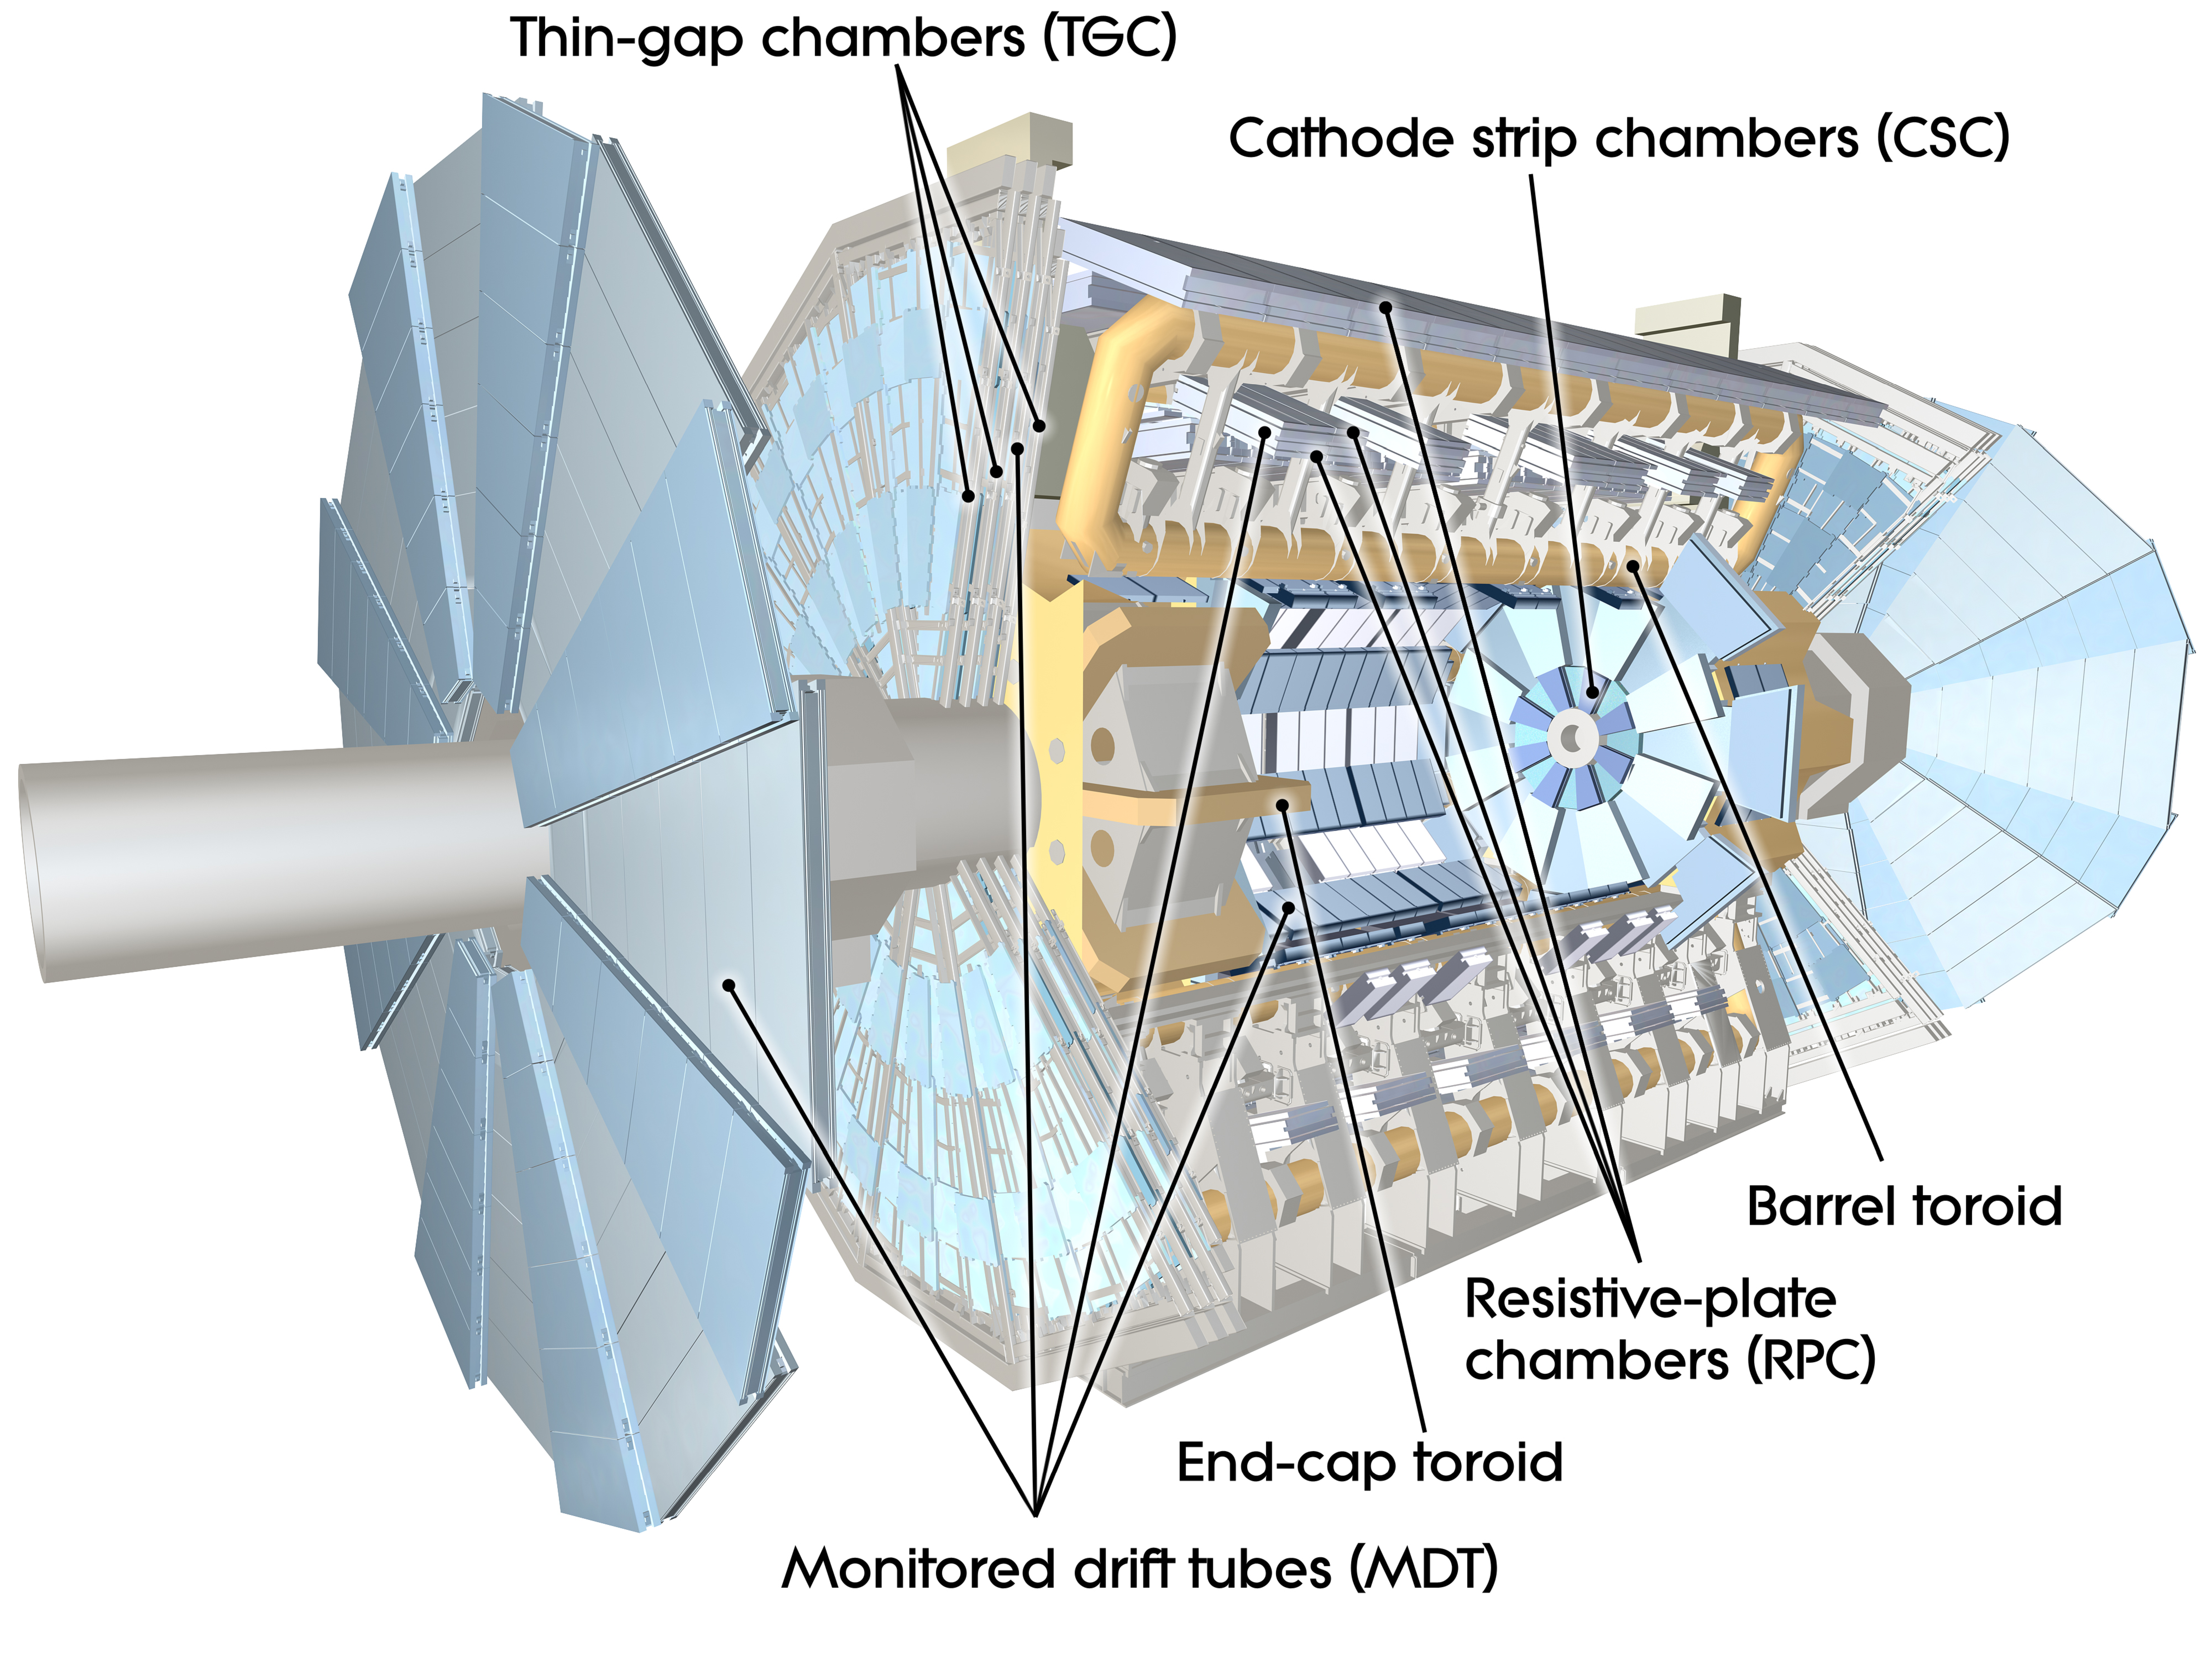
\includegraphics[width=0.8\textwidth]{fig/detector/muon_system.pdf}
    \caption[]{}
\label{chap:detector:fig:muon_system}
\end{figure}

\subsection{High precision tracking chambers}

The precision tracking system consists of three (four) layers of
chambers in the barrel (end-cap) that are immersed in a toroidal
magnetic field. In the barrel, there are eight toroidal magnetic coils
positioned symmetrically in $\phi$, and for each coil, there is a pair
of chambers. The chamber pairs form an alternating set of large and
small rectangular chambers, with adjacent chambers overlapping in $\phi$ to
minimize acceptance loss. In the end-caps, each wheel is also composed
of overlapping large and small chambers, but the geometry of the
chambers is trapezoidal. 

Two precision tracking technologies have been adopted. The predominant
chamber type is the monitored drift tube chamber (MDT). These chambers
contain parallel 3.0~cm copper tubes that run parallel to the $\phi$
direction in both the barrel and end-caps. Inside of the tube is a 50
\micron tungsten-rhenium wire at 3080~V that collects the ionization
electrons from interactions between incident muons and the ArCO$_2$
gas between the tube and the anode. Tubes are arranged into layers and
segmented in $\eta$ and $\phi$. Parallel tubes are separated by a
distance of 60 \micron. The spatial resolution of an MDT is limited by
the degree to which the position of the tube is known. Each chamber is
equipped with an internal optical alignment system capable of
measuring deformations at the level of a few \micron. Morever, to
avoid resolution degradation due to a sagging anode wire, which is
expected to be \textapprox{1~mm}, the tension of the wire can be
adjusted. The resulting spatial resolution of a single tube is 80
\micron. 

In the inner region of the first end-cap layer, the counting rate
exceeds the limit for MDTs, and therefore another chamber
technology, the cathode strip chamber (CSC), is introduced. These
chambers span the region $2.0 < |\eta| < 2.7$ and have the same
alternating large and small plate configuration as the end-cap
MDTs. Each chamber contains four layers of side-by-side parallel anode
wires with the central wire oriented radially. The cathodes, which are
2.5~mm from the wire plane, are strips on either side of the wires
forming two plans. In one plane, the strips run perpindicular to the
wires, providing a precision spatial measurement in the bending
direction. The other cathode has strips running parallel to the wires
and is segmented more coarsely. With this configuration, the CSC
provides four two-dimensional measurements with a spatial resolution
of 40 \micron in one direction and 5~mm in the other. Moreover, the
temporal resolution is about 7~ns per plane. This makes bunch-crossing
identification possible in a high particle density environment. 

\subsection{Trigger chambers}

The muon trigger system is an important component of the muon
spectrometer. It is designed to (1) discriminate muons based on
tranverse momentum, (2) associate a muon with a particular bunch
crossing, (3) provide fast and coarse tracking for high level triggers
(see section~\ref{chapter:detector:section:trigger}), (4) give another
spatial measurement to complement the MDT, and (5) be robust against
neutron and photon backgrounds~\cite{bib:Aad:2008zzm}. Due to the fact
that the environments are quite different in the barrel and end-caps,
two different technologies are in place in these regions. 

In the barrel region ($|\eta| < 1.05$), three layers of resistive
plate chambers (RPCs) form the trigger system. Two of the layers
sandwich the second MDT layer while the third is located immediately
in front of, or behind, the last MDT layer. Each RPC has two 2~cm drift layers with
parallel plates and a series of strips positioned such that both
$\phi$ and $\eta$ are measured. In each of the end-caps, where
backgrounds are more problematic, thin gap chambers (TGCs) are used
instead of RPCs. There is one TGC layer in front of the second MDT
wheel, two behind the same wheel, and a fourth layer immediately in
front of the first tracking chamber layer. Each chamber in the TGC
system has two or three drift layers, each providing an independent
measurement of $R$ and $\phi$. A drift layer consists of two parallel
graphite plates that are parallel to the $x$-$y$ plane. Between the
plates are parallel anode wires that run tangential to $phi$ in the
center of the chamber. The gaseous ionizing medium is a mixture of CO$_2$ and
n-pentane. On the sides of the plates that do not face the anodes,
copper strips that are in contact with the graphite and run tangent to
$R$ allow the azimuthal coordinate to be read out. 


\section{Trigger System}
\label{chapter:detector:section:trigger}

Due to limited resources, it is not possible to store the information
associated with each collision event at the design collision rate of
1~GHz. The trigger system selects potentially interesting events,
thereby reducing the effective collision rate, before events are
stored for downstream analysis. It is organized into three levels---
Level-1 (L1), Level-2 (L2), and event filter (EF). This three level
structure seeks to deal with a
fundamental problem of selecting potentially interesting events,
namely that such a decision requires partial event reconstruction,
which by its nature, requires time and memory. The levels progress
from very fast and coarse reconstruction applied to events which are
collected at a high rate to a more refined reconstruction
applied to a small subset of these events. 

The L1 trigger integrates a limited amount of information from all of
the calorimeter
subsystems and the muon trigger chambers to identify high
\et~electrons, photons, jets, and muons. The calorimeter trigger
system searches for energy deposits in a coarse granularity cell of
$\Delta\eta \times \Delta\phi = 0.1 \times 0.1$ that fall above a
series of configured thresholds. If the multiplicity of these deposits
falls above an energy-threshold-dependent cut-off value, then the
event passes the trigger. The muon trigger system uses RPC (TGC)
measurements in the barrel (end-caps) to identify patterns that are
consistent with a muon originating from the collision point. Starting
with a muon hit in the second chamber layer, the trigger searches for
additional hits along a path formed by extrapolating to the collision
point, and if a minimum number of hits is found, the pattern is
considered a muon candidate. If the number of muon candidates for the
same bunch crossing falls above a threshold, the L1 muon trigger is
accepted. The trigger is binned into 6 transverse momentum bins. The
L1 trigger reduces the event rate from 1~GHz to 75~kHz with each
trigger decision executed in less than $2.5 \mu$s. L1 trigger
processing is done in the front-end electronics system on the
detector, as is the storage of event data in buffers. Once the L1
trigger is passed, the data are sent away from the detector to readout
drivers, awaiting the L2 trigger. 

The L2 trigger is considered a high level trigger (HLT) in that it makes a
trigger decision based on the full granularity of the detector and
even some information from the ID. As opposed to the L1 triggers that
use front-end hardware to process an event, the L2 trigger system is
built around a specialized software-based framework that runs on a
computer farm. L2 triggers consider small event data fragments
associated with regions of interest (ROIs) that are defined by the L1
trigger. Data for each ROI is typically on the order of 1\% of the
total data in the event, which speeds up the L2 trigger processing and
minimizes the amount of data transferred to the farm. The L2 trigger
algorithms iteratively pull data from the readout drivers and determine
whether an ROI satisfies the hypothesis for a given particle. If the
algorithm determines that the ROI is not consistent with a particle,
the next ROI data is pulled and the process repeats. If none of the
ROIs are found to be consistent with particles, the event is
rejected. In its current form, the L2 system can only accomodate an
event rate of 40~kHz, about half of the design trigger rate for the L1
trigger. L2 further reduces the trigger rate to 3.5~kHz, with a
processing time of around 40~ms for each event. 

The final trigger level is the event filter (EF) trigger. It is also a
HLT, but instead of using full granularity portions of the event (ROIs), it
improves on the L2 trigger by incorporating all of the event data into
the processing algorithms. Event processing is done offline in
computer clusters at an average rate of four seconds
per event, and the resulting trigger rate is reduced to 200~Hz. Events
that pass the EF trigger are transferred to the CERN computer center
for permanent storage. The raw data for each event amounts to around
1.3~MB on average. 





